\section{Eiffage table plan}
\label{eiffageTablePlan}

%TODO Afficher des plans
\begin{figure}[h]
    \centering
    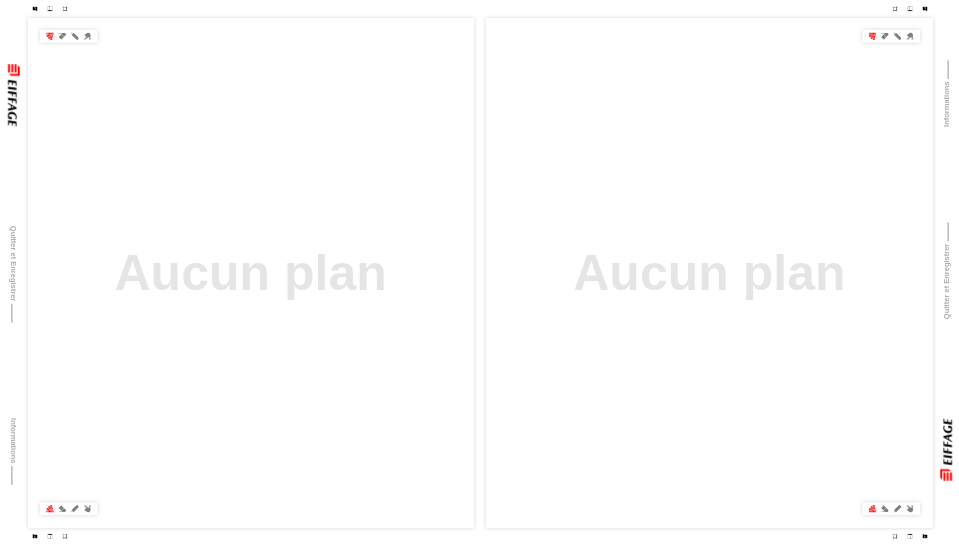
\includegraphics[scale=0.5]{img/table-plan-capture.png}
    \caption{Capture d'écran de l'application Table Plan}
\end{figure}

Dans le trio d'applications de la nouvelle salle cokpit d'Eiffage, l'application d'édition de plan m'a été accordée en partie.
L'objectif de cette application est d'afficher et de permettre la manipulation de plans (au format PDF) issus de  l'espace réseau d'Eiffage.
Cette application est affichée sur un ecran intègré dans une table faite sur mesures permettant l'interaction de plusieurs personnes au même moment.

Le cahier des charge de cette application est le suivant :
\begin{itemize}
    \item Charger et afficher des plans depuis le réseau d'Eiffage
    \item Permettre aux utilisateurs de manipuler les plans affichés
    \item Permettre aux utilisateurs d'annoter les plans affichés et d'enregistrer ces annotations pour les transmettre à l'archithecte
    \item Utiliser un design compatible avec l'affichage sur une table tactile ou plusieurs personnes sont assises autour d'un écran affichant l'application.
\end{itemize}

\subsection{Application existante}
\label{eiffageTablePlanApplicationExistante}

Cette application était la plus avencée des trois lors du début du projet.
L'équipe précédente avait beaucoup travaillé sur l'affichage des PDF.

En effet, les PDF de Eiffage sont très lourds et demandent un affichage particulier.
L'équipe ayant travaillé sur ce projet a donc beaucoup réfléchis à la technologie à utiliser pour afficher les PDF sans ralentissements.
Ils ont donc opté pour une apploche orientée Web avec un chargement, non pas du PDF en lui même, mais d'une image de ce PDF rendue a l'aide de ImageMagick.
Ils ont alors utilisé PixiJs, une librairie 2D pour WebGL, pour afficher l'image du PDF et permettre l'annotation.

Le plus gros de l'application, l'edition de plan, etait déjà codée et j'ai donc eu l'objectif de créer l'interface pour qu'elle reflète les creations du designer.
Mais aussi que l'application soit utilisable en collaboration et donc autour d'une table.

En revanche, l'ancienne application n'utilisait pas les WebComponents et j'ai du m'adapter pour reformer le code présent.
De plus, le développeur me précédent, n'avait pas dutout les même habitudes de développement et la même structure que moi et j'ai donc eu une longue phase d'analyse pour comprendre le rôle de chaque élément.

\subsection{Technologie}
\label{eiffageTablePlanTechnologie}

Les technologies utilisés dans le cadre de ce projet sont les même que les autres applications de ce type crées par LTBL.
On y retrouve Electron pour l'affichage de l'application et les Webcomponents pour la structcure interne.

\subsection{Structure}
\label{eiffageTablePlanStructure}

L'application se divise alors en de multiples WebComponents chacun ayant un rôle spécifique.
Dans ce projet j'ai éxpérimenté sur l'utilisation de Stores permettant le stockage des données de l'application pour une sychronisation des différents éléments.

\begin{figure}[h]
    \centering
    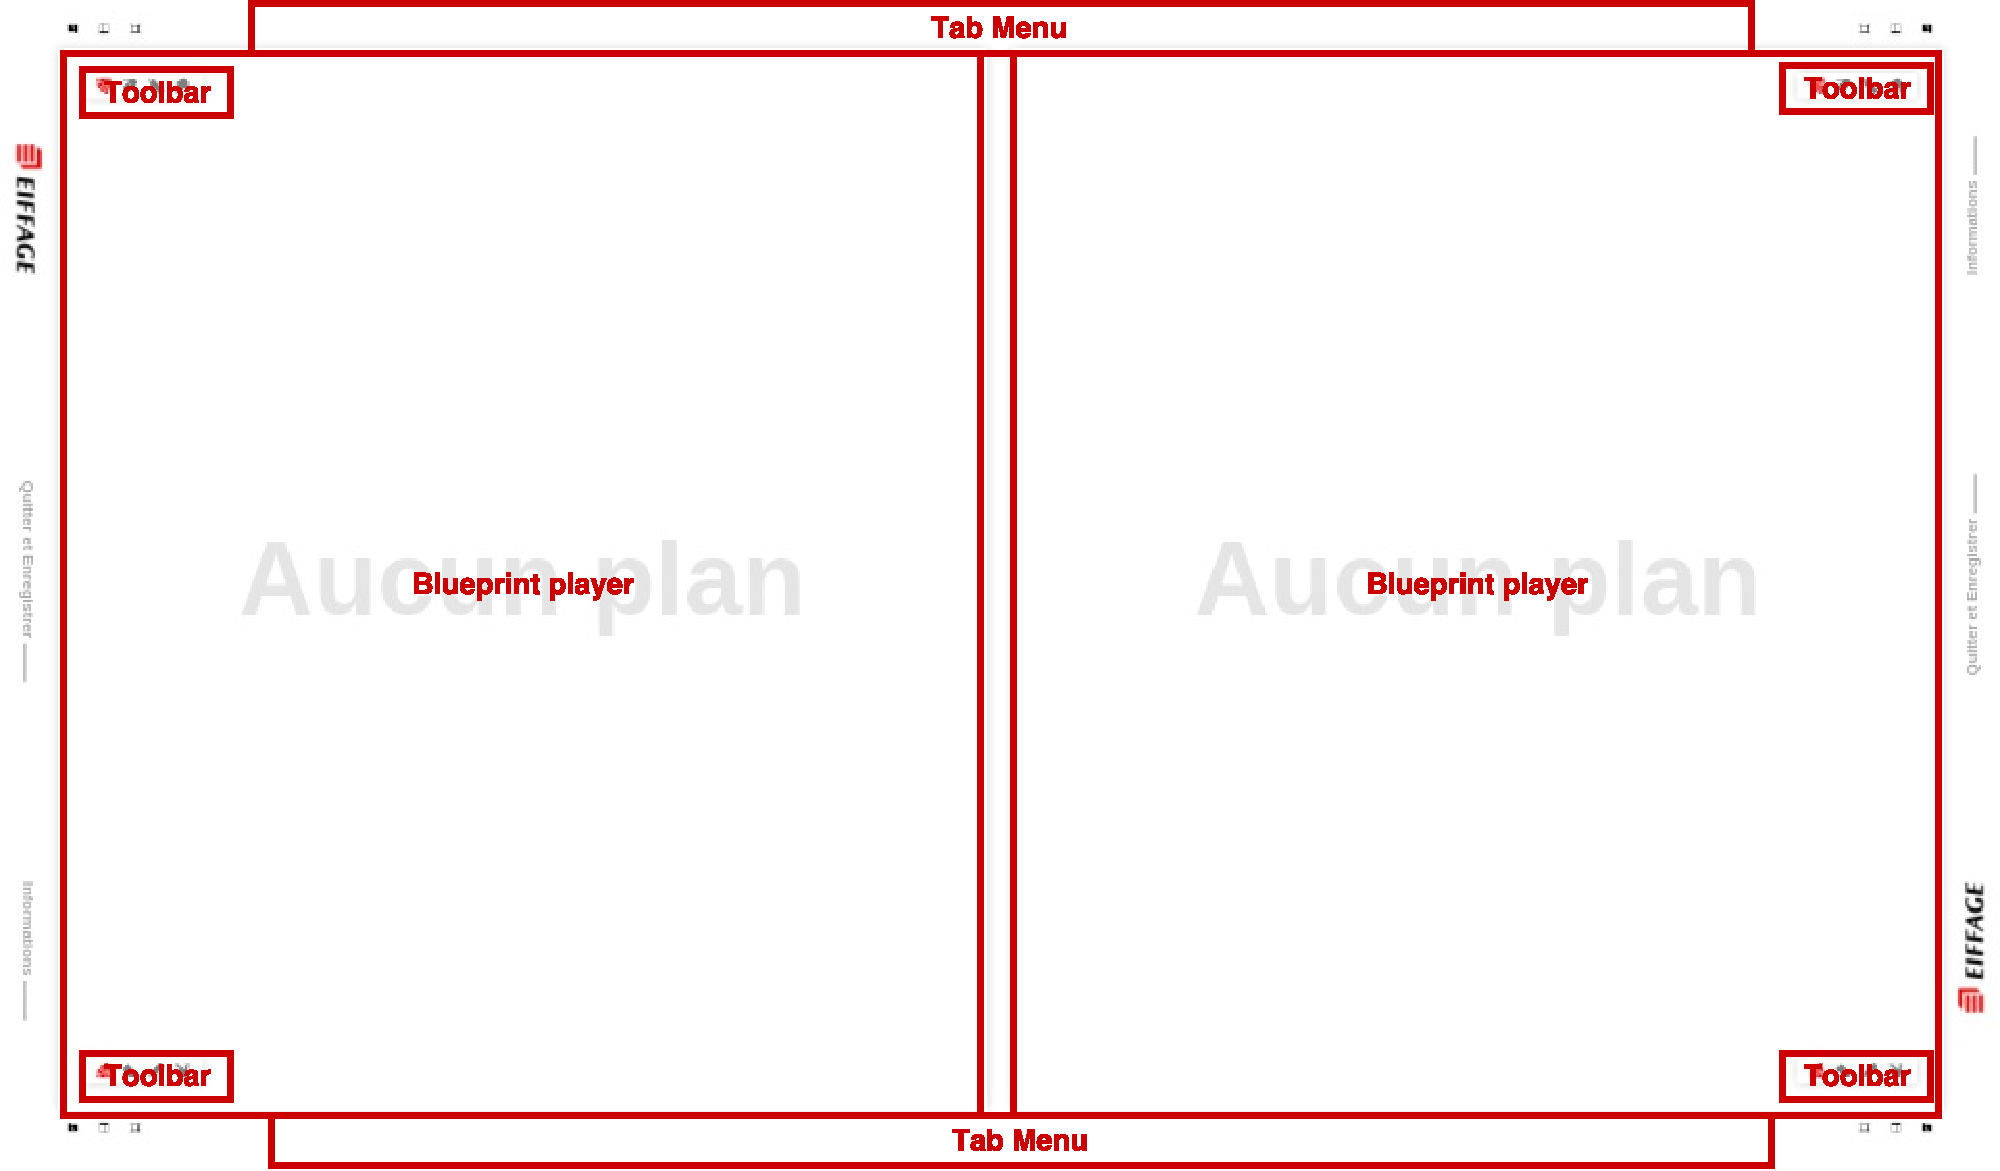
\includegraphics[scale=0.5]{img/table-plan-structure.pdf}
    \caption{Structure de l'application Table Plan}
\end{figure}

\subsubsection{Stores}
\label{eiffageTablePlanStores}

%TODO parler des stores

\subsection{Style}
\label{eiffageTablePlanStyle}

L'un des points majeurs de cette mission fut le style de l'application.
En effet, on est loin d'une application standard éxécutée sur un bureau.
On remarque que l'utilisation faite de cette application nécéssite une mise en place particulière des éléments de l'interface.

On remarque notemment que les barres d'outils sont présentes au 4 coins de l'interfaces toutes dirigés vers l'exterieur de l'application pour permettre an'importe quel collaborateur autour de la table d'interagir avec les plans.
Cela a demandé la mise en place d'une synchronisation des barres d'outils au niveau de l'application et l'utilisation de propriétés CSS de transformations a des fins bien plsu ergonomiques qu'esthetiques.

\bigskip

On remarque aussi que la barre des onglets ouverts est aussi inversé sur la partie superieur de l'application.
Cela a demandé une modification au niveau du code lui même car je ne pouvais pas me contenter d'éffectuer un mirroir sur l'élément (ce que j'ai fait pour les barres d'outils).
La raison de cette spécificité est la présence de texte.
Mettre un effet de mirroir sur un texte le rend completement illisible (contrairement à un icone) et j'ai éfféctué une rotation au lieu de faire un mirroir.
Mais cela posé d'autres problèmes puisque la droite et la gauche etait inverée sur chacun des éléments.
J'ai donc modifié le code source du composant de la barre d'onglets pour qu'elle inverse toutes les commandes dans certains cas.

\subsection{Conversion}
\label{eiffageTablePlanConversion}

Les plans d'Eiffage etant très lourds, ils sont impossible à ouvrir tel quel dans l'application.
Il faut donc utiliser un logiciel de conversion pour rendre les PDF sous forme d'image.

Les PDF de plans d'eiffage etant des plans vectoriels\footnote{Une image vectorielle est une image dont on ne spécifie pas la couleur de chaque pixel mais on spécifie une suite d'instruction permettant de calculer l'image finale. Les fichiers PDF, AI et SVG sont des exemples de fichiers vectoriels} ils nécéssitent un calcul préalable pour les afficher.
Pour résoudre le problème de loudeur des fichiers, j'ai mis en place un système de conversion automatique des plans.

\bigskip

Des qu'un fichier PDF est ouvert, on vérifie dans un dossier de cache s'il n'est pas déjà converti.
Si il l'es, on ouvre simplement la conversion précédente.
S'il ne l'est pas, on lance un conversion.
On informa alors l'utilisateur de la conversion en cours et on attend la fin de cette conversion avant d'ouvrir le fichier converti.

\begin{figure}[h]
    \centering
    
\includegraphics[scale=0.3]{img/image-magick.png}
    \hspace{5cm}
    
\includegraphics[scale=0.13]{img/ghostscript.png}
    \caption{Les logis de ImageMagick (à gauche) et GhostScript (à droite)}
\end{figure}

La conversion est effectuée avec ImageMagick, un logiciel de manipulation d'images très performant, et de GhostScript, un logiciel permettant de rendre des fichiers PDF avec ImageMagick.

Pour permettre un rendu optimal dans toutes les circonstances, nous avons choisi de rendre les plans en 4K et de les afficher dans une fenètre 4 fois superieur a leur taille pour avoir une trai d'annotation fin bien défini.